% (c) Nikita Lisitsa, lisyarus@gmail.com, 2024

\documentclass[10pt]{beamer}

\usepackage[T2A]{fontenc}
\usepackage[russian]{babel}
\usepackage{minted}

\usepackage{graphicx}
\graphicspath{ {./images/} }

\usepackage{adjustbox}

\usepackage{color}
\usepackage{soul}

\usepackage{hyperref}

\usetheme{metropolis}

\definecolor{red}{rgb}{1,0,0}
\definecolor{green}{rgb}{0,0.5,0}
\definecolor{blue}{rgb}{0,0,1}
\definecolor{codebg}{RGB}{29,35,49}
\definecolor{lightbg}{RGB}{253,246,227}
\setminted{fontsize=\footnotesize}

\makeatletter
\newcommand{\slideimage}[1]{
  \begin{figure}
    \begin{adjustbox}{width=\textwidth, totalheight=\textheight-2\baselineskip-2\baselineskip,keepaspectratio}
      \includegraphics{#1}
    \end{adjustbox}
  \end{figure}
}
\makeatother

\title{Я просто хотел писать игры}
\subtitle{Неожиданная математика в разработке игр}
\author{Никита Лисица}
\date{2024}
\titlegraphic{\vspace{4cm}\flushright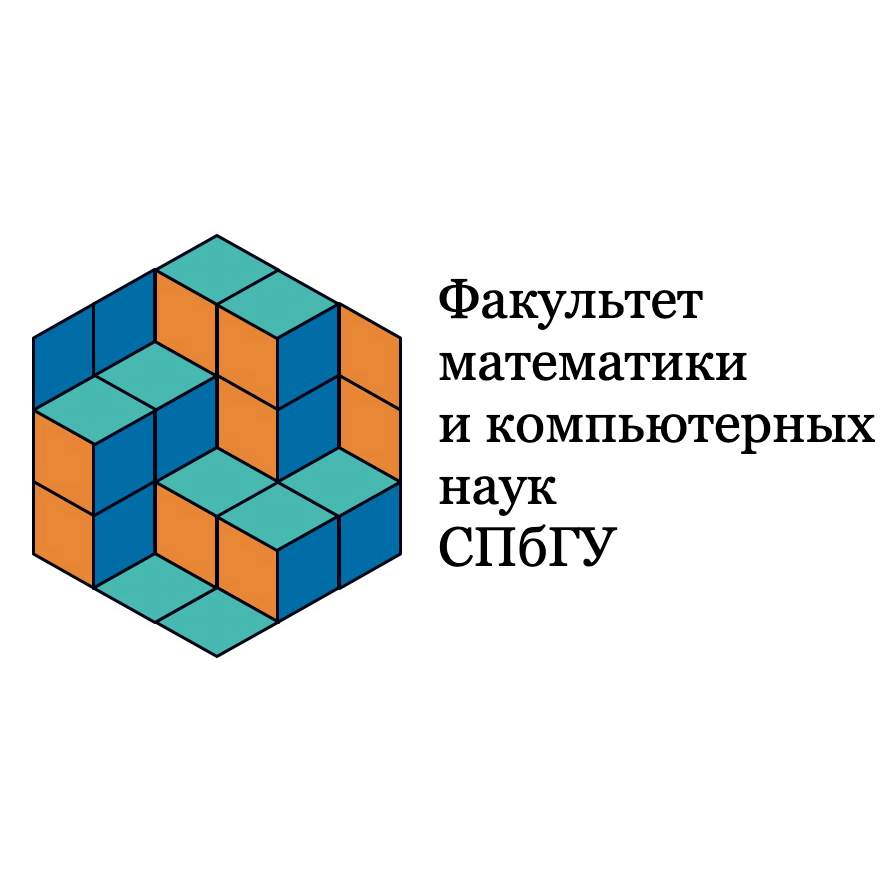
\includegraphics[width=0.5\textwidth]{fmkn.png}}

\setbeamertemplate{footline}[frame number]

\begin{document}

\frame{\titlepage}

\begin{frame}
\frametitle{Обо мне}
\begin{itemize}
\item Работаю в Яндекс Картах
\pause
\item Веду два спецкурса о комьютерной графике на факультете МКН в СПбГУ
\pause
\item В свободное время делаю инди-игры на собственном движке
\end{itemize}
\end{frame}

\begin{frame}
\frametitle{Яндекс.Карты}
\slideimage{maps.png}
\end{frame}

\begin{frame}
\frametitle{Курс о real-time графике}
\slideimage{realtime.png}
\end{frame}

\begin{frame}
\frametitle{Курс о трассировке лучей}
\slideimage{raytracing.png}
\end{frame}

\begin{frame}
\frametitle{Инди-игры}
\slideimage{game1.png}
\end{frame}

\begin{frame}
\frametitle{Инди-игры}
\slideimage{game2.png}
\end{frame}

\begin{frame}
\frametitle{Из чего состоят игры?}
Разработка игр -- очень сложный, мультидисциплинарный вид деятельности:
\pause
\begin{itemize}
\item Программирование логики
\pause
\item Графический движок
\pause
\item Физика
\pause
\item Аудио
\pause
\item Создание контента (моделей, текстур, анимаций, эффектов)
\pause
\item Гейм-дизайн
\pause
\item ...и многое другое
\end{itemize}
\pause
Где здесь нужна математика? \pause Практически везде!
\end{frame}

\begin{frame}
\frametitle{Перемещение персонажа}
\slideimage{character_move.png}
\end{frame}

\begin{frame}
\frametitle{Перемещение персонажа}
\begin{itemize}
\item Игрок нажал клавишу влево/вправо/вверх/вниз -- что нужно сделать в коде игры?
\pause
\item Сдвинуть положение персонажа на какой-то \textit{вектор}!
\pause
\item \begin{math}\text{position}_1 = \text{position}_0 + \text{move}\end{math}
\pause
\item Например, для перемещения влево \begin{math}\text{move} = (-1, 0)\end{math}
\pause
\item Персонаж резко переместится в другое место -- это некрасиво!
\end{itemize}
\end{frame}

\begin{frame}
\frametitle{Плавное перемещение персонажа}
\begin{itemize}
\item Сделаем перемещение анимированным!
\pause
\item Анимация -- зависимость чего-либо от времени, часто в виде явно заданной функции
\pause
\item \begin{math}\text{position}(t) = \text{position}_0 + \delta(t) \cdot \text{move}\end{math}, где
\begin{gather*}
\delta : [0, 1] \rightarrow [0, 1] \\
\delta(0) = 0 \\
\delta(1) = 1
\end{gather*}
\pause
\item Такие функции \begin{math}\delta\end{math} обычно называют \textit{easing} функциями
\end{itemize}
\end{frame}

\begin{frame}
\frametitle{Easing функции}
\begin{itemize}
\item \begin{math}\delta(t) = t\end{math} -- движение с постоянной скоростью
\pause
\item \begin{math}\delta(t) = t^2\end{math} -- движение с постепенным ускорением, начинающееся плавно и резко заканчивающееся
\pause
\item \begin{math}\delta(t) = 1-(1-t)^2\end{math} -- движение с постепенным замедлением, начинающееся резко и плавно заканчивающееся
\pause
\item \begin{math}\delta(t) = 3t^2-2t^3\end{math} -- движение, начинающееся и заканчивающееся плавно (\textit{smoothstep})
\end{itemize}
\end{frame}

\begin{frame}
\frametitle{Smoothstep}
\slideimage{smoothstep.png}
\end{frame}

\begin{frame}
\frametitle{Smoothstep}
\begin{itemize}
\item Smoothstep -- \begin{math}s(t) = 3t^2-2t^3\end{math} -- очень важная функция!
\pause
\item Настолько важная, что она встроена во все языки шейдеров, и про неё есть отдельная статья на википедии
\pause
\item Это многочлен минимальной степени, удовлетворяющий условиям
\begin{equation*}
s(0) = 0 \quad s(1) = 1 \quad s'(0) = 0 \quad s'(1) = 0
\end{equation*}
\pause
\item Эта функция часто используется для анимаций и сглаживания
\end{itemize}
\end{frame}

\begin{frame}
\frametitle{Генерация мира}
\slideimage{minecraft.png}
\end{frame}

\begin{frame}
\frametitle{Генерация мира}
\begin{itemize}
\item Многие современные игры используют \textit{процедурную генерацию контента (PCG)}, в том числе для генерации всего игрового мира
\pause
\item Есть много подходов к генерации мира, но грубо их можно разделить на два: \textit{глобальный} и \textit{локальный}
\pause
\item В глобальном подходе генерируется сразу весь мир -- например, целый остров с горами, реками, и поселениями
\pause
\item В локальном подходе мир генерируется постепенно, и различные его участки могут генерироваться независимо друг от друга
\pause
\item Для игр с очень большим миром предпочтительнее \textit{локальный подход}
\end{itemize}
\end{frame}

\begin{frame}
\frametitle{Генерация мира}
\slideimage{minecraft-chunk.png}
\end{frame}

\begin{frame}
\frametitle{Генерация мира}
\begin{itemize}
\item Итак, мы хотим сгенерировать небольшой кусочек нашего мира
\pause
\item Для простоты будем считать, что мы хотим только сгенерировать высоту ландшафта в каждой точке, т.е. \textit{карту высот}
\pause
\item Для этого нам нужен \textit{шум}
\end{itemize}
\end{frame}

\begin{frame}
\frametitle{Шум}
\slideimage{white-noise.png}
\end{frame}

\begin{frame}
\frametitle{Шум}
\begin{itemize}
\item В игровой индустрии \textit{шумом} называют любую функцию, выглядящую случайной
\pause
\item Часто, эта функция задана не для непрерывного аргумента, а на дискретной сетке
\pause
\item \textit{Белый шум} -- шум, значения которого в разных ячейках сетки никак не зависят друг от друга
\pause
\item Такой шум плохо подходит для карты высот!
\end{itemize}
\end{frame}

\begin{frame}
\frametitle{Карта высот на основе белого шума}
\slideimage{white-noise-terrain.png}
\end{frame}

\begin{frame}
\frametitle{Гладкий шум}
\begin{itemize}
\item Нам нужен какой-нибудь \textit{непрерывный шум} -- плавно меняющаяся, но всё ещё случайная функция
\pause
\item Один из самых распространённых алгоритмов для этого называется \textit{шумом Перлина} (по фамилии его изобретателя, Кена Перлина)
\end{itemize}
\end{frame}

\begin{frame}
\frametitle{Гладкий шум}
\begin{itemize}
\item Этот алгоритм генерирует случайные единичные векторы в вершинах квадратной сетки
\pause
\item Для получения значения шума в некоторой точке, алгоритм вычисляет скалярные произведения этих векторов с векторами из точки в вершины сетки, и затем интерполирует их
\end{itemize}
\end{frame}

\begin{frame}
\frametitle{Шум Перлина: векторы}
\slideimage{perlin-noise-vectors.png}
\end{frame}

\begin{frame}
\frametitle{Шум Перлина: скалярные произведения}
\slideimage{perlin-noise-dot.png}
\end{frame}

\begin{frame}
\frametitle{Шум Перлина}
\begin{itemize}
\item Получив четыре скалярных произведения \begin{math}d_1,\dots,d_4\end{math} из ближайших вершин сетки, алгоритм интерполирует между ними, используя координаты в ячейке сетки как коэффициенты интерполяции
\pause
\item Если точка в квадрате (ячейке сетки) имеет координаты \begin{math}x, y \in [0, 1]\end{math}, то значение шума алгоритм вычисляет с помощью \textit{билинейной интерполяции}
\begin{equation*}
x\cdot y\cdot d_1 + (1-x)\cdot y \cdot d_2 + x \cdot (1-y) \cdot d_3 + (1-x) \cdot (1-y)\cdot d_4
\end{equation*}
\end{itemize}
\end{frame}

\begin{frame}
\frametitle{Шум Перлина: билинейная интерполяция}
\slideimage{perlin-noise-lerp.png}
\end{frame}

\begin{frame}
\frametitle{Шум Перлина}
\begin{itemize}
\item У полученного шума явно видна исходная сетка, и он мало пригоден для использования
\pause
\item На помощь приходит уже известная нам функция \textit{smoothstep}: нужно просто применить её к коэффициентам интерполяции!
\end{itemize}
\pause
\begin{gather*}
x \leftarrow 3x^2 - 2x^3 \\
y \leftarrow 3y^2 - 2y^3
\end{gather*}
\end{frame}

\begin{frame}
\frametitle{Шум Перлина}
\slideimage{perlin-noise.png}
\end{frame}

\begin{frame}
\frametitle{Фрактальный шум}
\begin{itemize}
\item Такой шум лучше, чем белый шум, но он всё ещё слишком плавный
\pause
\item Обычно для генерации ландшафта смешивают несколько слоёв такого шума с разными размерами сетки
\pause
\item Получающийся шум называют \textit{фрактальным шумом}
\end{itemize}
\end{frame}

\begin{frame}
\frametitle{Фрактальный шум}
\slideimage{fractal-noise.png}
\end{frame}

\begin{frame}
\frametitle{Фрактальный шум}
\begin{itemize}
\item Значение шума можно взять в качестве высоты ландшафта в точке
\pause
\item На основе шума, или комбанации нескольких слоёв шума, можно построить карты температуры, количества осадков, и т.п.
\end{itemize}
\end{frame}

\begin{frame}
\frametitle{Карта на основе фрактального шума}
\slideimage{fractal-map.png}
\end{frame}

\begin{frame}
\frametitle{Рассчёт освещения}
\begin{itemize}
\item Сейчас наша карта выглядит плоской
\pause
\item Чтобы передать её трёхмерность, нужно применить к ней \textit{освещение}
\pause
\item Чтобы вычислить освещённость поверхности, нужно знать, насколько сильно она повёрнута в сторону света
\pause
\item За это отвечает вектор \textit{нормали} \begin{math}n\end{math} -- перпендикуляр к поверхности объекта
\end{itemize}
\end{frame}

\begin{frame}
\frametitle{Нормаль}
\slideimage{normal-vectors.png}
\end{frame}

\begin{frame}
\frametitle{Вычисление нормали}
\begin{itemize}
\item Для поверхности, заданной своей функцией высоты от точки \begin{math}z(x,y)\end{math} вектор нормали вычисляется на основе \textit{частных производных}
\pause
\begin{equation*}
n = \frac{\left(-\frac{\partial z}{\partial x}, -\frac{\partial z}{\partial y}, 1\right)}{\sqrt{1+\left(\frac{\partial z}{\partial x}\right)^2+\left(\frac{\partial z}{\partial y}\right)^2}}
\end{equation*}
\pause
\item Значит, нам нужно посчитать производную от шума Перлина!
\end{itemize}
\end{frame}

\begin{frame}
\frametitle{Частные производные}
\slideimage{perlin-gradient.png}
\end{frame}

\begin{frame}
\frametitle{Карта нормалей}
\slideimage{perlin-normal.png}
\end{frame}

\begin{frame}
\frametitle{Нормаль к шуму Перлина}
\begin{itemize}
\item Снова явно видна исходная сетка, по которой строился шум, но почему?
\pause
\item Изначально мы видели сетку из-за того, что функция шума была непрерывной, но \underline{не была} непрерывной \textit{её производная}
\pause
\item Человеческий глаз очень хорошо видит разрывы в первой производной :)
\end{itemize}
\end{frame}

\begin{frame}
\frametitle{Разрыв в производной}
\slideimage{plot.png}
\end{frame}

\begin{frame}
\frametitle{Разрыв в производной}
\slideimage{gradient.png}
\end{frame}

\begin{frame}
\frametitle{Нормаль к шуму Перлина}
\begin{itemize}
\item Мы избавились от видимой сетки, применив функцию \textit{smoothstep}, у которой производные на концах отрезка \begin{math}[0, 1]\end{math} равны нулю
\pause
\item Освещение зависит от вектора нормали, а вектор нормали зависит от производной нашей функции
\pause
\item Значит, чтобы убрать видимую сетку на нормалях, нужно сделать непрерывной \textit{вторую производную}!
\pause
\item Для этого есть функция \textit{smootherstep}: \begin{math}s(x)=6x^5-15x^4+10x^3\end{math}
\end{itemize}
\end{frame}

\begin{frame}
\frametitle{Плавные нормали}
\slideimage{perlin-normal-smooth.png}
\end{frame}

\begin{frame}
\frametitle{Карта с освещением}
\slideimage{perlin-shading.png}
\end{frame}

\begin{frame}
\frametitle{Ландшафт на основе фрактального шума}
\slideimage{perlin-noise-terrain.png}
\end{frame}

\begin{frame}
\frametitle{Физический движок}
\slideimage{physics.png}
\end{frame}

\begin{frame}
\frametitle{Физический движок}
\begin{itemize}
\item Задача физического движка -- симулировать физические взаимодействия между объектами
\pause
\item Например, движение твёрдого тела описывается приложенными к нему силами \begin{math}F\end{math} и уравнением Ньютона \begin{math}F = ma\end{math}
\pause
\item Ускорение -- это вторая производная от положения объекта \begin{math}\frac{d^2}{dt^2}q\end{math}
\pause
\item Физическому движку нужно решать \textit{дифференциальное уравнение}!
\end{itemize}
\pause
\begin{equation*}
\frac{d^2}{dt^2}q = \frac{F}{m}
\end{equation*}
\end{frame}

\begin{frame}
\frametitle{Физический движок}
\begin{itemize}
\item Обычно силы, приложенные к объектам, зависят от действий игрока
\pause
\item Обычно объектов в мире довольно много
\pause
\item Нет смысла решать физические уравнения \textit{аналитически} (в виде явной формулы), лучше решать их \textit{численно и приближённо}, используя \textit{дискретные шаги во времени}
\end{itemize}
\end{frame}

\begin{frame}
\frametitle{Физический движок}
\begin{itemize}
\item Есть много разных методов численного решения уравнений движения: явный и неявный методы Эйлера, симплектический метод Эйлера, методы Рунге-Кутты, и т.д.
\pause
\item Например, симплектический метод Эйлера выглядит так:
\begin{gather*}
v_1 = v_0 + \frac{F}{m} \cdot \Delta t \\
p_1 = p_0 + v_1 \cdot \Delta t
\end{gather*}
\pause
\item Он прост в реализации и хорошо сохраняет энергию физической системы
\end{itemize}
\end{frame}

\begin{frame}
\frametitle{Методы решения уравнений движения}
\slideimage{integrators.png}
\end{frame}

\begin{frame}
\frametitle{Вращения}
\begin{itemize}
\item Хочется, чтобы объекты не только двигались, но и \textit{вращались}!
\pause
\item Как описать вращение объекта?
\pause
\item В 2D это сделать несложно: вращение можно описать одним углом поворота
\pause
\item В 3D всё становится куда веселее!
\end{itemize}
\end{frame}

\begin{frame}
\frametitle{Трёхмерные вращения}
\slideimage{euler_angles.png}
\end{frame}

\begin{frame}
\frametitle{Трёхмерные вращения}
\begin{itemize}
\item Можно описать трёхмерное вращения тремя \textit{углами Эйлера}
\pause
\item С этими углами очень неудобно работать!
\pause
\item Можно описать вращение матрицей \begin{math}3\times 3\end{math}
\pause
\item С матрицами очень удобно работать, но они крайне избыточны (нужно запомнить 9 значений вместо 3), и не любая матрица является вращением
\end{itemize}
\end{frame}

\begin{frame}
\frametitle{Кватернионы}
\begin{itemize}
\item Решение -- \textit{кватернионы}!
\pause
\item Кватернионы -- это четвёрки вещественных чисел \begin{math}(x,y,z,w)\end{math} с покомпонентным сложением и хитрым, некоммутативным законом умножения
\pause
\item \textit{Что-то вроде} четырёхмерных комлексных чисел
\pause
\item Очень интересный и важный математический объект
\end{itemize}
\end{frame}

\begin{frame}
\frametitle{Кватернионы}
\begin{itemize}
\item Через кватернионы можно выразить любое вращение трёхмерного вектора \begin{math}v\end{math} с помощью некоторого кватерниона \begin{math}q\end{math} и формулы
\begin{equation*}
v \mapsto q\cdot v \cdot q^{-1}
\end{equation*}
\pause
\item Абсолютно все игровые движки используют кватернионы!
\end{itemize}
\end{frame}

\begin{frame}
\frametitle{Распространение света}
\begin{itemize}
\item Основная задача компьютерной графики -- описать и смоделировать \textit{распространение света}
\pause
\item Свет взаимодействует с объектами по очень сложным законам
\pause
\item В общем случае свет, выходящий из какой-то точки объекта в каком-то направлении, складывается из света, пришедшего \textit{из всех возможных направлений}!
\pause
\item Чтобы это смоделировать, нужно использовать \textit{интегральный уравнения}
\end{itemize}
\end{frame}

\begin{frame}
\frametitle{Распространение света}
\slideimage{rendering_equation.png}
\end{frame}

\begin{frame}
\frametitle{Уравнение рендеринга}
\begin{equation*}
\hspace*{-0.5cm}
{\color{magenta}I_{out}}(p, {\color{magenta}\vec\omega_{out}}, \lambda) = I_{e}(p, {\color{magenta}\vec\omega_{out}}, \lambda)+\int\limits_{\mathbb S^2} {\color{blue}I_{in}}(p, {\color{blue}\vec\omega_{in}}, \lambda) \cdot {\color{green}f}(p, {\color{blue}\vec\omega_{in}}, {\color{magenta}\vec\omega_{out}}, \lambda) \cdot ({\color{blue}\vec\omega_{in}} \cdot \vec{n}) d{\color{blue}\vec\omega_{in}}
\end{equation*}
\hspace*{-0.5cm}
\pause
\begin{itemize}
\item \begin{math}{\color{magenta}I_{out}}\end{math} -- количество света, выходящего из точки
\pause
\item \begin{math}I_{e}\end{math} -- количество излучаемого света 
\pause
\item \begin{math}{\color{blue}I_{in}}\end{math} -- количество света, приходящего в точку 
\pause
\item \begin{math}{\color{green}f}\end{math} -- функция, описывающая материал объекта
\end{itemize}
\end{frame}

\begin{frame}
\frametitle{Уравнение рендеринга}
\begin{equation*}
\hspace*{-0.5cm}
{\color{magenta}I_{out}}(p, {\color{magenta}\vec\omega_{out}}, \lambda) = I_{e}(p, {\color{magenta}\vec\omega_{out}}, \lambda)+\int\limits_{\mathbb S^2} {\color{blue}I_{in}}(p, {\color{blue}\vec\omega_{in}}, \lambda) \cdot {\color{green}f}(p, {\color{blue}\vec\omega_{in}}, {\color{magenta}\vec\omega_{out}}, \lambda) \cdot ({\color{blue}\vec\omega_{in}} \cdot \vec{n}) d{\color{blue}\vec\omega_{in}}
\end{equation*}
\hspace*{-0.5cm}
\pause
\begin{itemize}
\item Описывает многие визуальные эффекты: тени, отражение, преломление, рассеяние света
\pause
\item \textit{Очень сложно} решать!
\pause
\item Один из моих курсов \textit{целиком} про это уравнение :)
\end{itemize}
\end{frame}

\begin{frame}
\frametitle{Уравнение рендеринга}
\slideimage{bunny.png}
\end{frame}

\begin{frame}
\frametitle{Уравнение объёмного рендеринга}
\begin{itemize}
\item Обычное уравнение рендеринга описывает только взаимодействие света с \textit{поверхностью} объектов
\pause
\item Многие эффекты требуют взаимодействия света с \textit{объёмом}: туман, лучи света в пыльной комнате, и даже цвет самого неба
\pause
\item Для этого нужно ещё более сложное \textit{уравнение объёмного рендеринга}!
\end{itemize}
\end{frame}

\begin{frame}
\frametitle{Уравнение объёмного рендеринга}
\begin{gather*}
I(p+L\omega,\omega) = I(p,\omega)\exp\left(-\int\limits_0^L k_a(p+t\omega)dt\right) +\\
+ \int\limits_0^L k_e(p+t\omega) \exp\left( -\int\limits_t^L k_a(p+s\omega)ds \right)dt
\end{gather*}
\end{frame}

\begin{frame}
\frametitle{Уравнение объёмного рендеринга}
\begin{itemize}
\item Часто используется в медицине -- например, для визуализации МРТ-обследований
\pause
\item Используется в играх для `объёмных' лучей света, тумана, облаков, или для реалистичного неба
\end{itemize}
\end{frame}

\begin{frame}
\frametitle{Лучи света}
\slideimage{light-shaft.png}
\end{frame}

\begin{frame}
\frametitle{Небо}
\slideimage{sky.png}
\end{frame}

\end{document}